\section{Banco de Dados}

Como requisito funcional é necessário armazenar as informações de modo não volátil, optou-se por utilizar um banco de dados relacional. Devido a praticidade encontrada e conhecimento prévio do autor, a tecnologia utilizada para tal foi a do \textit{MySQL}.

Para a realização de um registro de ponto eletrônico, duas entidades estão envolvidas: a pessoa responsável por registrar o ponto, e o próprio ponto. A relação é de 1-n, ou seja: uma pessoa pode ter múltiplos pontos, mas um ponto pode pertencer a apenas uma pessoa.

Cada pessoa possui um nome e uma foto, e é identificada unicamente por sua tag (o número de série de seu cartão ponto). Cada registro de ponto possui um identificador único de chave primária, uma tag referenciando uma pessoa, e a data e hora que o ponto foi registrado. A figura ~\ref{diagrama_er} demonstra as relações citadas.

\begin{figure}[h]
	\centering
	\caption{Diagrama de Entidade-Relacionamento do Banco de Dados.}
	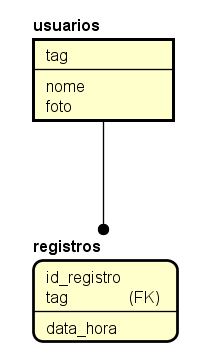
\includegraphics[scale=1]{imagens/bd_diagrama_er.png}
	\label{diagrama_er}
\end{figure}

Os tipos de dados foram escolhidos de modo a simplificar sua implementação em outras plataformas. Veja abaixo o \textit{script} de criação do banco de dados.

\renewcommand{\lstlistingname}{Código}
\begin{lstlisting}[language=SQL, label=bd_criacao, caption=Código de criação do banco de dados.]
DROP DATABASE IF EXISTS ponto;
CREATE DATABASE ponto;
USE ponto;

-- TABELA usuarios
DROP TABLE IF EXISTS usuarios;
CREATE TABLE usuarios (
 tag VARCHAR(10) NOT NULL,
 nome VARCHAR(64) NOT NULL,
 foto VARCHAR(256) NOT NULL,
 PRIMARY KEY (tag)
);

-- TABELA registros
DROP TABLE IF EXISTS registros;
CREATE TABLE registros (
 id_registro INT NOT NULL AUTO_INCREMENT,
 tag VARCHAR(10) NOT NULL,
 data_hora TIMESTAMP,
 PRIMARY KEY (id_registro),
 FOREIGN KEY (tag) REFERENCES usuarios (tag)
);
\end{lstlisting}